\documentclass[]{article}


\usepackage{amsmath}
\usepackage{cmap}
\usepackage[utf8]{inputenc}
\usepackage[russian]{babel}
\usepackage[left=1.5cm,right=1.5cm,top=2cm,bottom=2.5cm]{geometry}

\usepackage[fontsize=13pt]{scrextend}

% что-то за межстрочный интервал отвечающее
\renewcommand{\baselinestretch}{1.3}

\usepackage[nooneline]{caption}

\usepackage{indentfirst}
\usepackage{tabularx}


\usepackage{hyperref}



\usepackage{fancyhdr}


\setlength{\headheight}{15mm}


\usepackage[pdftex]{graphicx}
\graphicspath{{/home/maxim/Projects/Vega/Finance Econometrics/Project1/Plots}}

\pagestyle{fancy}
\lhead{\textbf{\normalsize Проект 1}}
\rhead{\textbf{\normalsize Выполнили: }\normalsize Кирякин Максим, Куренкова Дарья, Коваль Наталия}



\begin{document}

{
	\Large
	\href{https://github.com/MaximKiryakin/Vega/tree/FinanceEconometrics/Project1}{Репозиторий проекта}.
}

\section{Постановка задачи}

В работе было необходимо построить прогноз значений временного ряда с помощью моделей эконометрики, рассмотренных в курсе.

Модель ARIMA(p,d,q) -- это расширение моделей типа ARMA на нестационарные временные ряды, которые однако могут стать стационарным после применения процедуры дифференцирования ряда. Модель ARIMA(p, d, q) для ряда $y_t$ определяется как модель ARMA(p,q) для ряда разностей порядка d ряда $y_t$.

$\textbf{ARIMA(p, d, q)}$ модель:
\begin{equation*}
	\Delta^d y_t = \alpha_1 \Delta^d y_{t-1} + ... + \alpha_p\Delta^dy_{t-p} + \varepsilon_t + \beta_1\varepsilon_{t-1} + ... + \beta_q\varepsilon_{t-q},
\end{equation*}

где: $y_t$ -- значение временного ряда в момент времени $t$, $\Delta^d = (1 - L)^d$, $\varepsilon_t$ - белый шум. L - лаговый оператор.

Обобщение модели ARIMA на ряды с наличием сезонной составляющей назвается SARIMA. Пусть s — известная сезонность ряда. Добавим в модель ARIMA(p,d,q) компоненты, отвечающие за значения в предыдущие сезоны. Тогда модель SARIMA может быть записана следующим образом:

$\textbf{SARIMA(p, d, q)(P, D, Q)s}$ модель:

\begin{equation*}
	\begin{split}
		\Delta^D_s\Delta^d y_t 
		&= \alpha_1\Delta^D_s \Delta^d y_{t-1} + \dots + \alpha_p\Delta^D_s\Delta^dy_{t-p} \\
		&\quad+ \varepsilon_t + \beta_1\varepsilon_{t-1} + \dots + \beta_q\varepsilon_{t-q} \\
		&\quad+ \alpha_1^s\Delta^D_s \Delta^d y_{t-s} + \dots + \alpha_p^s\Delta^D_s \Delta^d y_{t-ps} \\
		&\quad+ \beta_1^s\varepsilon_{t-s}+\beta_Q^s\varepsilon_{t-Qs}.
	\end{split}
\end{equation*}

где: $\Delta^D_s = (1 - L^s)^D$



Обобщением SARIMA модели является SARIMAX модель.
SARIMAX (Seasonal AutoRegressive Integrated Moving Average with eXogenous inputs) – это эконометрическая модель для прогнозирования временных рядов с учетом сезонности и внешних факторов.


\section{Ход работы}
\subsection{Данные}

В работе решалась задача прогнозирования числа продаж в сети магазинов Эквадора за 2016 год. \href{https://www.kaggle.com/c/store-sales-time-series-forecasting/data}{Данные} были взяты с сайта Kaggle. Всего в работе использовались 3 файла (train.csv, stores.csv, oil.csv), на основе которых формировался итоговый датасет.

Описание значений переменных файла train.csv:
\begin{itemize}
	\item  $store\_nbr$ идентифицирует магазин, в котором продаются товары.  
	\item  $family$ определяет тип продаваемого продукта.  
	\item  $sales$ указывает общую сумму продаж для определенной группы товаров в конкретном магазине на заданную дату. Возможны дробные значения, так как товары могут продаваться в дробных единицах (например, 1,5 кг сыра вместо 1 пакета чипсов).  
	\item  $onpromotion$ указывает общее количество товаров в группе продуктов, которые были на акции в магазине на заданную дату.
\end{itemize}

Файл stores.csv содержит метаданные магазинов, включая город, штат, тип и кластер (все магазины были разбиты на группы по схожести). Файл oil.csv содержит ежедневные цены на нефть. Включает значения как в период обучения, так и в период тестирования. (Эквадор — страна, зависимая от нефти, и ее экономическое состояние сильно подвержено колебаниям цен на нефть.)

\subsection{Модели и их валидация}

Было рассмотрено 3 модели для прогнозирования временного ряда:
\begin{itemize}
	\item ARIMA модель с ручной настройкой параметров p, d и q
	\item SARIMAX модель
	\item Модель машинного обучения (градиентный бустинг XGBRegressor)
\end{itemize}


Качество оценивалось с помощью следующих метрик: MSE, RMSE, MAE, абсолютная процентная ошибка. Результаты сравнивались с наивным прогнозом -- средним числом продаж за последние 3 месяца. 

Для моделей SARIMAX и бустинга рассматривались два подхода. В первом случае в качестве переменных в модель подавались временные признаки: номера месяца, квартала, дня в году и недели, а также день недели.
Кроме этого, использовались <<лаговые переменные>>: число продаж в эту же дату год, два и три назад (если есть данные за этот период). Такой подход позволяет получать прогноз модели на любое число дней вперед. Во втором случае к этим переменным добавлялись переменные из датасета: цена на топливо за выбранную дату, число акций в магазинах и число транзакций. Трудность второго подхода заключается в том, что мы не знаем будущие значений добавленных драйверов заранее. Если мы хотим получить прогноз на даты, которых нет в нашем датасете, -- величины драйверов тоже придется предсказывать.

\subsection{Предварительная обработка данных}

Переменные датасета требовали предварительной предобработки. Например, в значениях цены на газ были пропуски, которые были заполнены с помощью интерполяции квадратичными сплайнами. На рисунках \ref{price_raw} и \ref{price_solid} приведены графики цены до интерполяции и после соответственно.

\begin{figure}[h!]
	\centering
	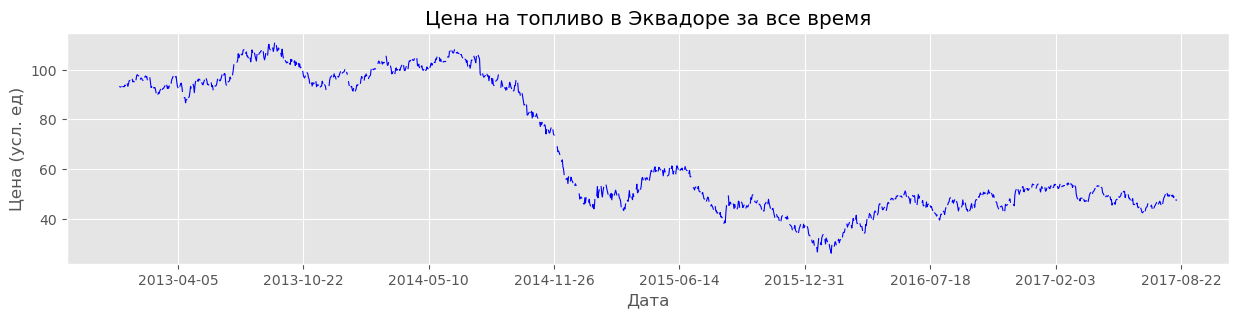
\includegraphics[width=1.\textwidth]{OilPrice.png}
	\caption{Цена за литр топлива в Эквадоре до интерполяции.}
	\label{price_raw}
\end{figure}


\begin{figure}[h!]
	\centering
	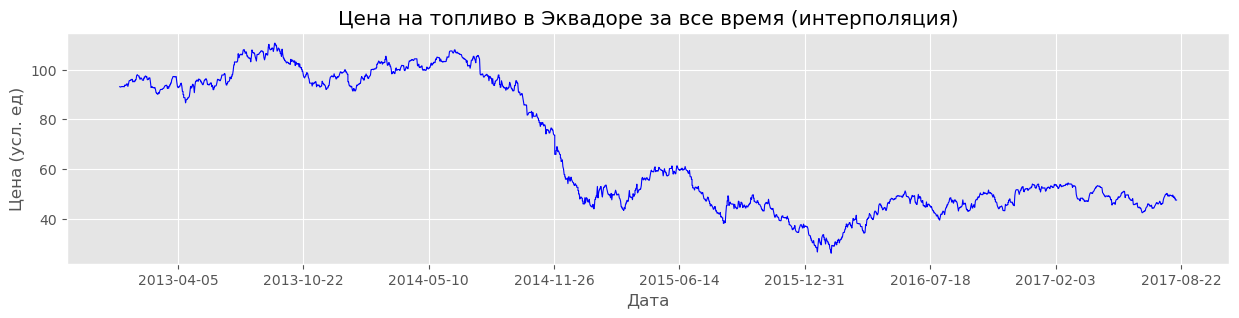
\includegraphics[width=1.\textwidth]{OilPriceEnterpolated.png}
	\caption{Цена за литр топлива в Эквадоре после интерполяции.}
	\label{price_solid}
\end{figure}

Кроме этого, категориальные переменные, такие как тип магазина, его локация и флаг праздничного дня, были закодированы числовыми значениями. Однако далее все эти признаки были исключены из модели из-за маленькой дисперсии (весь признак мог быть заполнен одним значением) или из-за их мальтиколлинеарности. Кроме того, для этих признаков наблюдалось большая доля пропусков, порядка 80 процентов.

\subsection{Обучение моделей}

\subsubsection{Наивный прогноз}

Как уже было описано ранее, для наивного прогноза использовалось среднее значение продаж в Эквадоре за последние 3 месяца 2016 года. График прогноза приведен на рисунке \ref{naive}.

\begin{figure}[h!]
	\centering
	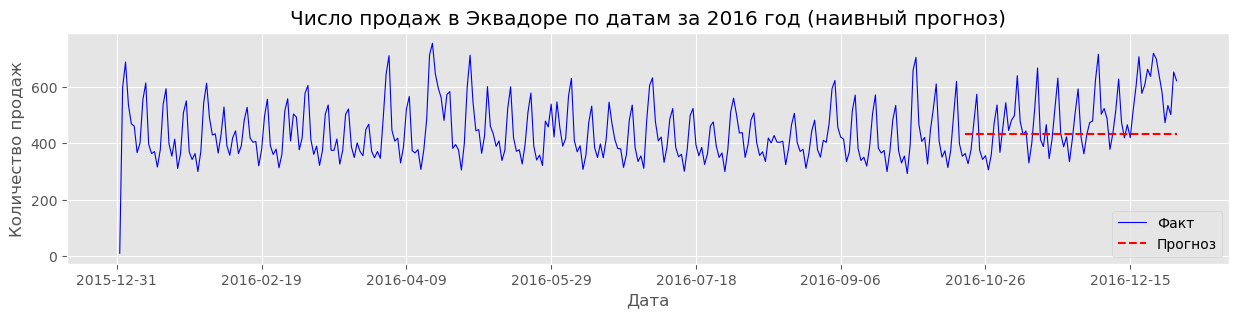
\includegraphics[width=1.\textwidth]{SalesNaive.png}
	\caption{Наивный прогноз для продаж в Эквадоре.}
	\label{naive}
\end{figure}

Для прогноза были измерены основные метрики. Их значения приведены в таблице \ref{tab:1}.

\begin{table}[h!]
	\centering
	\caption{Значения метрик на прогнозе модели градиентного бустинга.}
	\begin{tabularx}{\textwidth}{|X|l|l|l|l|}
		\hline
								& MSE       & RMSE   & MAE    & Процентная ошибка \\ \hline
		{Временные переменные}  & 20703.85  & 143.88 & 114.75 & 0.2               \\ \hline
	\end{tabularx}
	\label{tab:1}
\end{table}



\subsubsection{ARIMA модель}

Выбор параметров для ARIMA модели осуществлялся на основе значений функций автокорреляции и частичной автокорреляции. Стационарность ряда проверялась с помощью теста  Дики — Фуллера.

Было установлено, что исходный ряд не является стационарным ($p-value: 0.68$). После однократного дифференцирования ряд стал стационарным ($p-value: 6.33 \cdot 10^{-14}$). Кроме того, для ошибок был построен график их распределения, оно оказалось близко к нормальному. 

Результаты работы ARIMA модели проведены на рисунке \ref{fig:arima}.

\begin{figure}[h!]
	\centering
	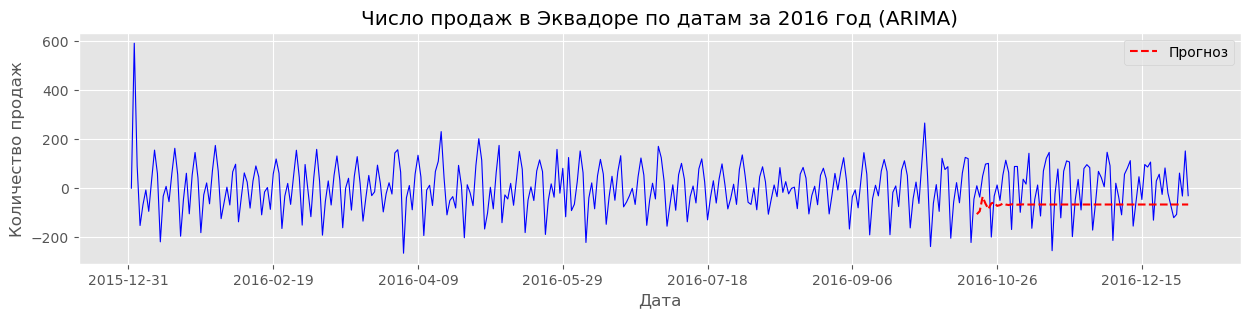
\includegraphics[width=1.\textwidth]{SalesARIMA.png}
	\caption{Прогноз ARIMA модели для числа продаж в Эквадоре.}
	\label{fig:arima}
\end{figure}

Из графика видно, что модель не улавливает динамику ряда и очень скоро прогноз превращается в константный. Значения метрик для ARIMA модели приведены в таблице \ref{tab:arima}.

\begin{table}[h!]
	\centering
	\caption{Значения метрик на прогнозе ARIMA модели.}
	\begin{tabularx}{\textwidth}{|X|l|l|l|l|}
		\hline
								& MSE       & RMSE   & MAE   & Процентная ошибка \\ \hline
		{Временные переменные}  & 11908.6   & 109.13 & 93.53 & 1.491             \\ \hline
	\end{tabularx}
	\label{tab:arima}
\end{table}



\subsubsection{SARIMAX модель}

Главное отличие SARIMAX модели от ARIMA модели -- ее способность учитывать сезонность в предсказании, а также дополнительные параметры, помимо значений самого ряда. Как уже было сказано выше, в качестве дополнительных параметров в модель подавались значения числа продаж в дату, цена топлива и числа акций в магазинах. Обучение модели проходило автоматически с помощью пакета $statsmodels$ языка Python. Кроме того, модель обучалась два раза: в первый раз -- только на временных и лаговых переменных, во второй -- с дополнительными переменными.
Результаты предсказания модели приведены на рисунке \ref{fig:sarimax}. Значения метрик представлены в таблице  \ref{tab:sarimax}.

\begin{figure}[h!]
	\centering
	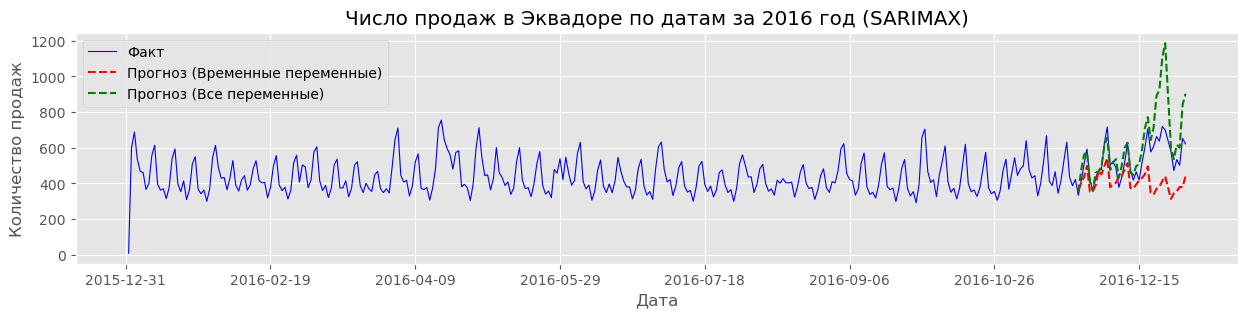
\includegraphics[width=1.\textwidth]{SalesSARIMAX.png}
	\caption{Прогноз SARIMAX модели для числа продаж в Эквадоре.}
	\label{fig:sarimax}
\end{figure}

\begin{table}[h!]
	\centering
	\caption{Значения метрик на прогнозе SARIMAX модели.}
	\begin{tabularx}{\textwidth}{|X|l|l|l|l|}
		\hline
		& MSE          & RMSE   & MAE   & Процентная ошибка \\ \hline
		{Временные переменные}                  & 24258.07 & 155.75 & 125.47 & 0.22\\ \hline
		{Временные переменные + дополнительные} & 19785.57 & 140.661   & 88.76 & 0.15 \\ \hline
	\end{tabularx}
	\label{tab:sarimax}
\end{table}

Из графика и значений метрик видно, что учет в модели дополнительных параметров дает значительный прирост в качетсве предсказания.


\subsubsection{Boosting}

В качестве дополнения к работе нам было интересно посмотреть, какие результаты покажет на тех же входных данных бустинг. Принцип работы бустинга принципиально отличается от эконометрических моделей, рассмотренных выше. 

В работе рассматривался XGBRegressor из библиотеки $sklearn$. Обучение также как и для SARIMAX модели осуществлялось двумя подходами. Перебор гиперпараметров осуществлялся с помощью библиотеки $hyperopt$. В отличии от обычного перебора по сетке, данный подход использует средства Байесовской оптимизации. Кроме того, при переборе гиперпараметров использовалась кросс-валидация, адаптированная под временные ряды.

Результаты предсказания модели приведены на рисунке \ref{fig:boosting}. Значения метрик представлены в таблице  \ref{tab:boosting}.

\begin{figure}[h!]
	\centering
	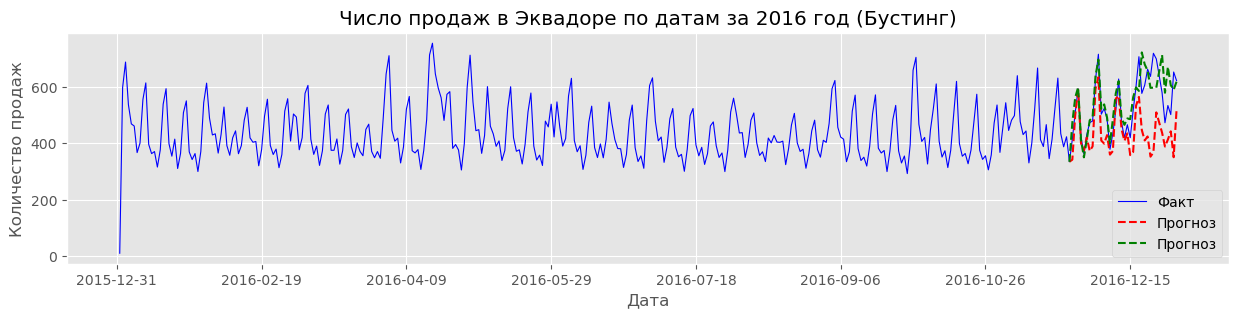
\includegraphics[width=1.\textwidth]{SalesBoosting.png}
	\caption{Прогноз модели градиентного бустинга для числа продаж в Эквадоре.}
	\label{fig:boosting}
\end{figure}

Из графика и значений метрик видно, что точность прогноза для спецификации с дополнительными переменными близка к реальным значениям числа продаж. 

\begin{table}[h]
	\centering
	\caption{Значения метрик на прогнозе модели градиентного бустинга.}
	\begin{tabularx}{\textwidth}{|X|l|l|l|l|}
		\hline
					& MSE          & RMSE   & MAE   & Процентная ошибка \\ \hline
		{Временные переменные}                  & 14971.71 & 122.36 & 86.83 & 0.15 \\ \hline
	    {Временные переменные + дополнительные} & 2745.55  & 52.4   & 39.19 & 0.07 \\ \hline
	\end{tabularx}
	\label{tab:boosting}
\end{table}

\newpage
\section{Заключение}

В работе была решена задача прогнозирования числа продаж в сети магазинов Эквадора за 2016 год. Было рассмотрено 3 способа прогнозирования:
\begin{itemize}
	\item ARIMA модель с ручной настройкой параметров p, d и q
	\item SARIMAX модель
	\item Модель машинного обучения (градиентный бустинг, XGBRegressor)
\end{itemize}

Было установлено, что среди эконометрических моделей лучше всего себя показала модель SARIMAX. Этот результат, в частности, обусловлен ее способностью учета внешних параметров, а не только прошлые значения ряда. 

Кроме того, в работе дополнительно был рассмотрен способ прогнозирования с помощью градиентного бустинга. Этот метод превзошел все эконометрические модели по качеству предсказаний. 
 
	
\end{document}
